\documentclass{article}[18pt]
\usepackage{../../../../format}
\lhead{Software Engineering}


\begin{document}
\begin{center}
\underline{\huge Modelling}
\end{center}
\section{System Modelling}
\begin{itemize}
	\item A model helps with getting an abstract idea of the objects that the software product will consist of and their interactions
	\begin{itemize}
		\item As such the point of view can shift dependent on your needs and the model you use
	\end{itemize}
	\item A model is easy to change
	\item Can be easily explained to non-technical audiences
	\item Can be used to measure against requirements (validation)
\end{itemize}
\section{The Unified Modelling Language}
\begin{itemize}
	\item UML is a diagrammatic language designed for OOP
	\item UML can describe:
	\begin{itemize}
		\item The organisation of the problem
		\item How a program executes
		\item How a program is used
		\item How a program is deployed over a network
		\item ... and others
	\end{itemize}
	\item UML can help with:
	\begin{itemize}
		\item Specification
		\item Visualisation
		\item Architecture design
		\item Construction
		\item Simulation and Testing
		\item Documentation
	\end{itemize}
	\item UML is comprised of multiple diagram types:
	\begin{center}
		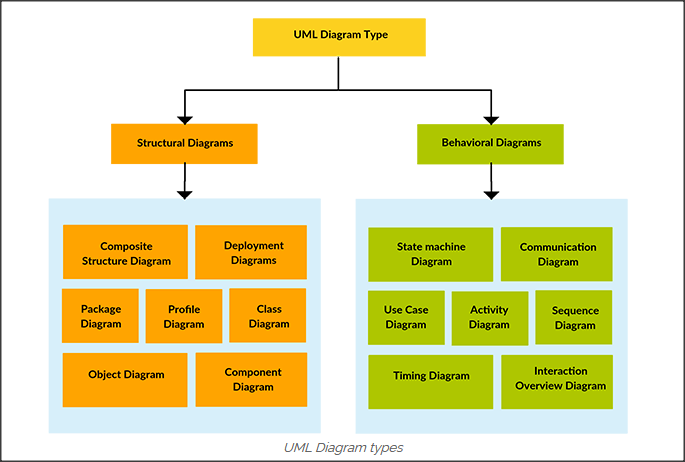
\includegraphics[scale=0.7]{UML}
	\end{center}
	\item Use case diagram
	\begin{center}
		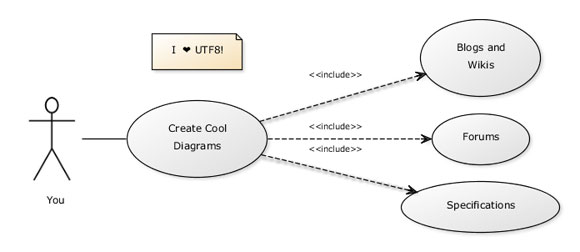
\includegraphics[scale=0.7]{UML1}
	\end{center}
	\begin{center}
		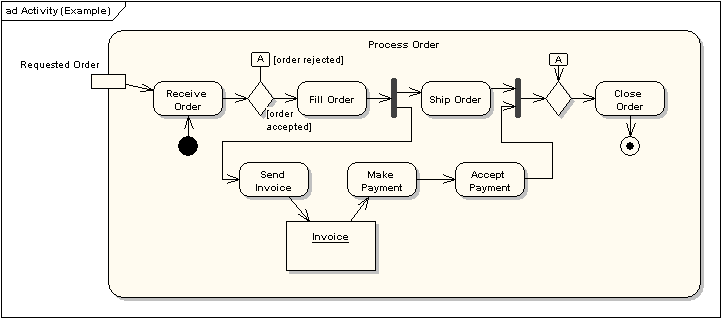
\includegraphics[scale=0.7]{UML2}
	\end{center}
\section{Class Diagrams}
\begin{center}
	\includegraphics[scale=0.7]{"Class Diagrams2"}
\end{center}

\begin{center}
	\includegraphics[scale=0.7]{"Class Diagrams1"}
\end{center}

\end{itemize}



\end{document}